\section{Objective}

\begin{frame}{Vision-Based Robotic Grasping of Diverse Objects}{}
    \centering
    \begin{columns}%
        \begin{column}{0.5\textwidth}%
            \centering
            \includegraphics[height=4.3cm]{graphics/setup_sketch.pdf}
        \end{column}
        %
        \begin{column}{0.5\textwidth}%
            \centering
            \includegraphics[height=4.3cm]{graphics/training_set.png}
        \end{column}
    \end{columns}
\end{frame}

\begin{frame}{Vision-Based Robotic Grasping of Diverse Objects}{Approach}
    \begin{columns}%
        \begin{column}{0.375\textwidth}%
            \begin{block}{Approaches}
                \begin{itemize}
                    \item Analytical
                    \item Empirical
                          \begin{itemize}
                              \item Supervised learning
                              \item Imitation learning
                              \item \only<1>{Reinforcement learning}\only<2>{\textbf{Reinforcement learning}}
                          \end{itemize}
                \end{itemize}
            \end{block}
        \end{column}
        %
        \begin{column}{0.625\textwidth}%
            \centering
            \onslide<2>{\includegraphics[width=\textwidth]{graphics/mdp_loop.pdf}}
        \end{column}
    \end{columns}
\end{frame}


\section{Task Definition}

\begin{frame}{Task Definition}{}
    \begin{columns}%
        \begin{column}{0.28\textwidth}%
            \begin{block}{Agent}
                \begin{itemize}
                    \item High-level controller
                          \begin{itemize}
                              \item Gripper pose
                              \item Gripper action
                          \end{itemize}
                \end{itemize}
            \end{block}
        \end{column}
        %
        \begin{column}{0.32\textwidth}%
            \begin{block}{Environment}
                \begin{itemize}
                    \item Objects
                    \item Robot
                          \begin{itemize}
                              \item Low-level controllers
                          \end{itemize}
                    \item Physics and visuals
                \end{itemize}
            \end{block}
        \end{column}
        %
        \begin{column}{0.35\textwidth}%
            \begin{block}{Episodic Task}
                \begin{itemize}
                    \item Success
                          \begin{itemize}
                              \item Lifting an object
                          \end{itemize}
                    \item Failure
                          \begin{itemize}
                              \item Pushing all objects away
                          \end{itemize}
                    \item Max 100 time steps
                          \begin{itemize}
                              \item \textasciitilde 40 s (simulation)
                          \end{itemize}
                \end{itemize}
            \end{block}
        \end{column}
    \end{columns}
\end{frame}

\begin{frame}{Task Definition}{Action Space}
    \begin{columns}%
        \begin{column}{0.4\textwidth}%
            \begin{block}{Actions in Cartesian Space}
                \begin{itemize}
                    \item Translational displacement
                          \begin{itemize}
                              \item \(d_{x}\)
                              \item \(d_{y}\)
                              \item \(d_{z}\)
                          \end{itemize}
                    \item Gripper rotation
                          \begin{itemize}
                              \item \(d_{\phi}\)
                          \end{itemize}
                    \item Gripper actions (open/close)
                          \begin{itemize}
                              \item \(g\)
                          \end{itemize}
                \end{itemize}
            \end{block}
        \end{column}
        %
        \begin{column}{0.6\textwidth}%
            \centering
            \includegraphics[height=6cm]{graphics/action_space.pdf}
        \end{column}
    \end{columns}
\end{frame}

\begin{frame}{Task Definition}{Observation Space}
    \begin{columns}%
        \begin{column}{0.6\textwidth}%
            \centering
            \only<1>{\includegraphics[height=6cm]{graphics/3d_data_representations.pdf}}\only<2->{\includegraphics[height=6cm]{graphics/3d_data_representations_only_octree.pdf}}
        \end{column}
        %
        \begin{column}{0.4\textwidth}%
            \onslide<3>{
                \begin{block}{Proprioceptive Observations}
                    \begin{itemize}
                        \item Gripper position
                        \item Gripper rotation
                        \item Gripper state
                    \end{itemize}
                \end{block}
            }
        \end{column}
    \end{columns}
    \only<1>{\footnoteref{}}\only<2->{\footnoteref{Wang et al. 2017. O-CNN: Octree-based Convolutional Neural Networks for 3D Shape Analysis. ACM Trans. Graph. (SIGGRAPH) 36, 4, Article 72.}}
\end{frame}

\begin{frame}{Task Definition}{Observation Space - Construction of Octree}
    \centering
    \includegraphics[width=\textwidth]{graphics/octree_creation_sketch.pdf}
\end{frame}

\begin{frame}{Task Definition}{Observation Space - Features and Stacks}
    \begin{columns}%
        \begin{column}{0.5\textwidth}%
            \begin{block}{Features}
                \begin{itemize}
                    \item Spatial
                          \begin{itemize}
                              \item Average normal vector \(\overline{n}\)
                              \item Average distance to points \(\overline{d}\)
                          \end{itemize}
                    \item Colour
                          \begin{itemize}
                              \item Average intensity of RGB channels \(\overline{rgb}\)
                          \end{itemize}
                \end{itemize}
            \end{block}
            \begin{block}{Observation Stacking}
                \begin{itemize}
                    \item Three consecutive observations
                \end{itemize}
            \end{block}
        \end{column}
        %
        \begin{column}{0.5\textwidth}%
            \centering
            \includegraphics[height=5cm]{graphics/octree_features_sketch.pdf}
        \end{column}
    \end{columns}
\end{frame}

\begin{frame}{Task Definition}{Reward Function}
    \begin{columns}%
        \begin{column}{0.5\textwidth}%
            \begin{block}{Composite Reward}
                \begin{itemize}
                    \item Reach
                          \begin{itemize}
                              \item \(+1\) (\(7^{0}\))
                          \end{itemize}
                    \item Touch
                          \begin{itemize}
                              \item \(+7\) (\(7^{1}\))
                          \end{itemize}
                    \item Grasp
                          \begin{itemize}
                              \item \(+49\) (\(7^{2}\))
                          \end{itemize}
                    \item Lift
                          \begin{itemize}
                              \item \(+343\) (\(7^{3}\))
                          \end{itemize}
                \end{itemize}
            \end{block}
        \end{column}
        %
        \begin{column}{0.5\textwidth}%
            \begin{block}{Recurring Reward}
                \begin{itemize}
                    \item Collision with ground/table
                          \begin{itemize}
                              \item \(-1\)
                          \end{itemize}
                    \item Incentive to act quickly
                          \begin{itemize}
                              \item \(-0.005\)
                          \end{itemize}
                \end{itemize}
            \end{block}
        \end{column}
    \end{columns}
\end{frame}

\begin{frame}{Task Definition}{Summary}
    \begin{columns}%
        \begin{column}{0.3\textwidth}%
            \centering
            \includegraphics[height=5cm]{graphics/3d_data_representations_only_octree_cropped.pdf}
        \end{column}
        %
        \begin{column}{0.3\textwidth}%
            \centering
            \includegraphics[height=4cm]{graphics/action_space.pdf}
        \end{column}
        %
        \begin{column}{0.35\textwidth}%
            \begin{block}{Reward Function}
                \begin{itemize}
                    \item Composite
                          \begin{itemize}
                              \item Reach
                              \item Touch
                              \item Grasp
                              \item Lift
                          \end{itemize}
                    \item Collision with ground/table
                    \item Incentive to act quickly
                \end{itemize}
            \end{block}
        \end{column}
    \end{columns}
\end{frame}


\section{Reinforcement Learning Algorithms and Network Architecture}

\begin{frame}{Reinforcement Learning}{Algorithms}
    \begin{columns}%
        \begin{column}{0.3\textwidth}%
            \begin{block}{Actor-Critic Algorithms}
                \begin{itemize}
                    \item TD3
                    \item SAC
                    \item TQC
                \end{itemize}
            \end{block}
            \begin{block}{Implementation}
                \begin{itemize}
                    \item Stable Baselines3
                \end{itemize}
            \end{block}
        \end{column}
        %
        \begin{column}{0.7\textwidth}%
            \centering
            \includegraphics[height=6cm]{graphics/actor_critic_loop.pdf}
        \end{column}
    \end{columns}
\end{frame}

\begin{frame}{Deep Reinforcement Learning}{Octree-Based Feature Extractor}
    \centering
    \includegraphics[width=\textwidth]{graphics/feature_extractor.pdf}
\end{frame}

\begin{frame}{Deep Reinforcement Learning}{Full Actor-Critic Network Architecture}
    \centering
    \includegraphics[width=\textwidth]{graphics/actor_critic_network_full.pdf}
\end{frame}


\section{Simulation Environment}

\begin{frame}{Simulation Environment}{Selection}
    \begin{columns}%
        \begin{column}{0.35\textwidth}%
            \begin{block}{Simulators}
                \begin{itemize}
                    \item MuJoCo
                    \item PyBullet
                    \item Gazebo Classic
                    \item \only<1>{Ignition Gazebo}\only<2>{\textbf{Ignition Gazebo}}
                    \item Isaac
                    \item Webots
                    \item Unreal Engine
                    \item Unity
                    \item Unigine
                    \item RaiSim
                    \item ...
                \end{itemize}
            \end{block}
        \end{column}
        %
        \begin{column}{0.65\textwidth}%
            \centering
            \onslide<2>{\includegraphics[width=0.65\textwidth]{graphics/ignition_logo.pdf}}
        \end{column}
    \end{columns}
\end{frame}

\begin{frame}{Simulation Environment}{Ignition Gazebo}
    \begin{columns}%
        \begin{column}{0.4\textwidth}%
            \begin{block}{Physics}
                \vspace{0.2cm}

                \centering
                \includegraphics[width=0.7\textwidth]{graphics/dart_logo.png}
            \end{block}

            \vspace{1cm}

            \begin{block}{Rendering}
                \vspace{0.2cm}

                \centering
                \includegraphics[width=0.7\textwidth]{graphics/ogre_logo.png}
            \end{block}
        \end{column}
        %
        \begin{column}{0.6\textwidth}%
            \onslide<2>{
                \begin{block}{Gym-Ignition}
                    \begin{itemize}
                        \item Interface for Ignition Gazebo
                        \item Tooling for creation of OpenAI Gym environments%
                              \begin{itemize}
                                  \item Compatibility with RL frameworks
                              \end{itemize}
                    \end{itemize}
                \end{block}
            }
        \end{column}
    \end{columns}
    \only<1>{\footnoteref{}}\only<2->{\footnoteref{Ferigo et al. 2020. Gym-Ignition: Reproducible Robotic Simulations for Reinforcement Learning. In 2020 IEEE/SICE International Symposium on System Integration (SII). 885–890.}}
\end{frame}

\begin{frame}{Simulation Environment}{Domain Randomisation}
    \centering
    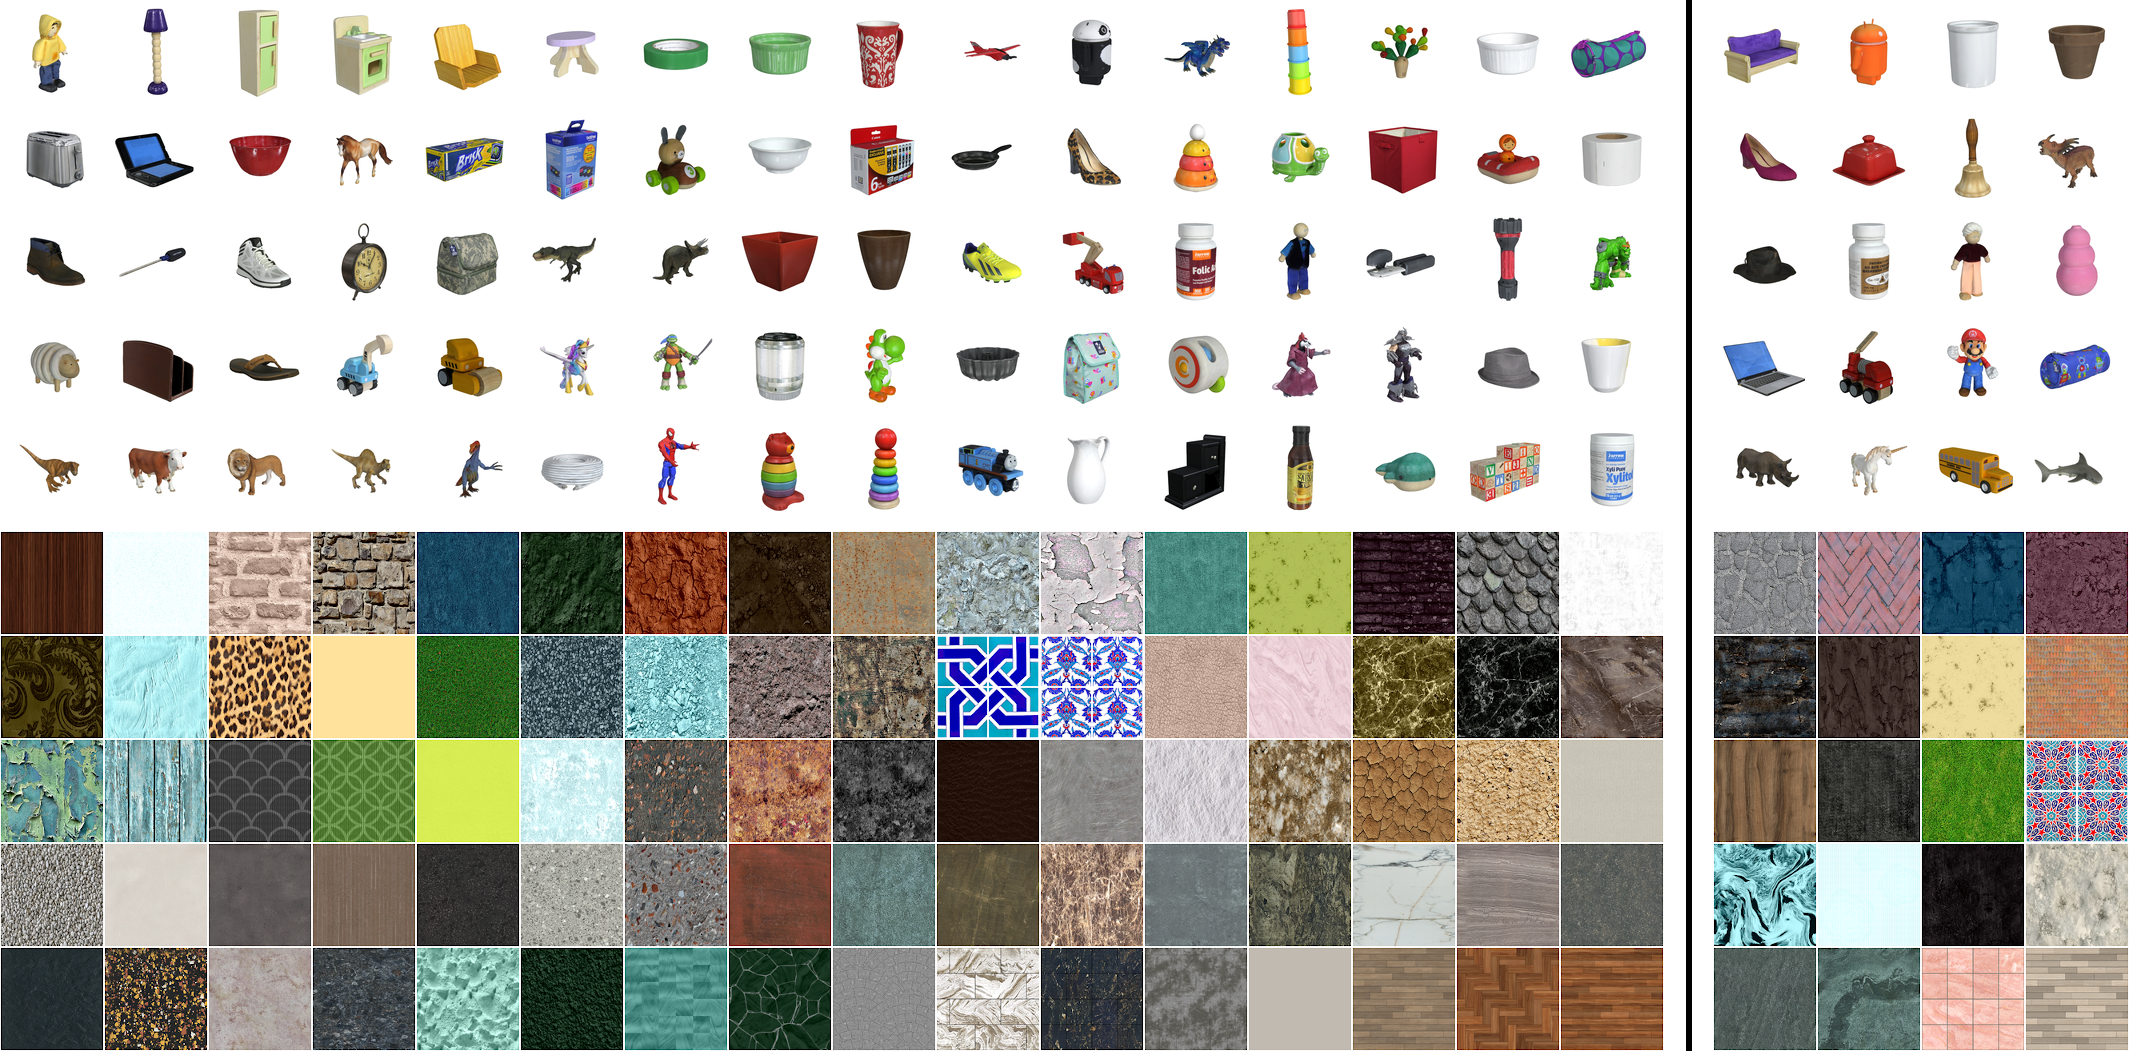
\includegraphics[height=6.5cm]{graphics/datasets_full.png}
\end{frame}

\begin{frame}{Simulation Environment}{Domain Randomisation}
    \centering
    \includegraphics[height=6.5cm]{graphics/domain_randomisation.png}
\end{frame}

\begin{frame}{Simulation Environment}{Domain Randomisation}
    \begin{columns}%
        \begin{column}{0.35\textwidth}%
            \begin{block}{Random}
                \begin{itemize}
                    \item Object
                          \begin{itemize}
                              \item Model
                              \item Scale
                              \item Mass
                              \item Friction
                              \item Pose
                          \end{itemize}
                    \item Ground plane texture
                    \item Initial robot configuration
                    \item Camera
                          \begin{itemize}
                              \item Pose
                              \item Sensory noise
                          \end{itemize}
                \end{itemize}
            \end{block}
        \end{column}
        %
        \begin{column}{0.65\textwidth}%
            \centering
            \includegraphics[height=4.75cm]{graphics/random_camera_pose.png}
        \end{column}
    \end{columns}
\end{frame}

\begin{frame}{Simulation Environment}{Environment for Training}
    \centering
    \only<1>{\includegraphics[height=6cm]{graphics/octree_example_1.pdf}}\only<2>{\includegraphics[height=6cm]{graphics/octree_example_2.pdf}}\only<3>{\includegraphics[height=6cm]{graphics/octree_example_3.pdf}}
\end{frame}

\begin{frame}{Training}{Hyperparameters}
    \begin{columns}%
        \begin{column}{0.3\textwidth}%
            \begin{block}{Optimisation}
                \begin{itemize}
                    \item Automatic (Optuna)
                    \item Manual
                \end{itemize}
            \end{block}
        \end{column}
        %
        \begin{column}{0.7\textwidth}%
            \centering
            \resizebox{0.85\textwidth}{!}{%
                \begin{tabular}{l|ccc}
                    \textbf{Hyperparameter}     & \textbf{TD3}                                                    & \textbf{SAC}                                 & \textbf{TQC} \\ \hline
                    Optimisation Algorithm      & \multicolumn{3}{c}{\begin{tabular}[c]{@{}c@{}}Adam\end{tabular}}                                                                                \\
                    Learning Rate Schedule      & \multicolumn{3}{c}{Linear, \(1.5 \cdot 10^{-4} \rightarrow 0\)}                                                               \\
                    Mini-batch Size             & \multicolumn{3}{c}{\(32\)}                                                                                                    \\
                    Update Frequency            & \multicolumn{3}{c}{After Every Episode}                                                                                       \\
                    Gradient Steps per Update   & \multicolumn{3}{c}{\(100\)}                                                                                                   \\
                    Replay Buffer Size          & \multicolumn{3}{c}{\(40000\)}                                                                                                 \\
                    Discount Factor \(\gamma\)  & \multicolumn{3}{c}{\(0.999\)}                                                                                                 \\
                    Target Update Rate \(\tau\) & \multicolumn{3}{c}{\(5 \cdot 10^{-5}\)}                                                                                       \\
                    Number of Critics           & \multicolumn{3}{c}{\(2\)}                                                                                                     \\
                    Activation Function         & \multicolumn{3}{c}{ReLU}                                                                                                      \\
                    Exploratory Action Noise    & \multicolumn{3}{c}{\(\mathcal{N}(0, 0.025)\)}                                                                                 \\ \hline
                    Target Policy Noise         & \(\mathcal{N}(0, 0.25)\)                                        & ---                                          & ---          \\ \hline
                    Initial Entropy Coefficient & ---                                                             & \multicolumn{2}{c}{\(0.1\)}                                 \\
                    Entropy Target              & ---                                                             & \multicolumn{2}{c}{\(-dim(\mathcal{A})=-5\)}                \\ \hline
                    Number of Atoms             & ---                                                             & ---                                          & \(25\)       \\
                    Number of Truncated Atoms   & ---                                                             & ---                                          & \(3\)        \\
                \end{tabular}
            }
        \end{column}
    \end{columns}
\end{frame}


\begin{frame}{Training}{Demonstrations and Curriculum}
    \begin{columns}%
        \begin{column}{0.5\textwidth}%
            \begin{block}{Demonstrations}
                \begin{itemize}
                    \item Automatic collection of samples
                          \begin{itemize}
                              \item Simple scripted policy
                                    \begin{itemize}
                                        \item 19\% success rate
                                    \end{itemize}
                          \end{itemize}
                    \item 5k Collected transitions
                          \begin{itemize}
                              \item Replaced after 40k steps (buffer size)
                          \end{itemize}
                \end{itemize}
            \end{block}
        \end{column}
        %
        \begin{column}{0.5\textwidth}%
            \begin{block}{Curriculum}
                \begin{itemize}
                    \item Scaling of environment difficulty
                          \begin{itemize}
                              \item Number of objects
                                    \begin{itemize}
                                        \item 1 \(\rightarrow\) 4
                                    \end{itemize}
                              \item Spawn area
                                    \begin{itemize}
                                        \item 2.4 cm\(\times\)2.4 cm \(\rightarrow\) 24 cm\(\times\)24 cm
                                    \end{itemize}
                          \end{itemize}
                    \item Full problem at 60\% success rate
                \end{itemize}
            \end{block}
        \end{column}
    \end{columns}
\end{frame}
